\section{Theorie}
\label{sec:Theorie}
\subsection{Der Doppler-Effekt}
Der Doppler-Effekt beschreibt die Frequenzänderung einer Welle bei
Relativbewegungen der Quelle und/oder des Beobachters.
\subsubsection{Ruhender Beobachter}
Bei Bewegung der Quelle zum Beobachter hin verschiebt sich die beobachtete
Frequenz zu höheren Frequenzen.
Wenn sich jedoch die Quelle vom Beobachter entfernt, verschiebt sich die
beobachtete Frequenz hin zu niedrigeren Frequenzen. Dieser Sachverhalt wird
beschrieben durch
\begin{equation*}
  \nu_{kl/gr} = \frac{\nu_0}{1 \mp \frac{\nu}{c}}.
\end{equation*}
Hierbei bezeichnet $\nu_0$ die weder gestauchte noch gestreckte Frequenz,
$\nu_{kl}$ die zu niedrigeren Frequenzen verschobene und $\nu_{gr}$ die zu höheren
Frequenzen verschobene Frequenz.
\subsubsection{Ruhende Quelle}
Bei Bewegung des Beobachters auf die Quelle zu erhöht sich die beobachtete Frequenz
$\nu_0$ auf höhere Frequenzen $\nu_h$.
Bei Bewegung des Beobachters von der Quelle weg verringert sich die beobachtete
Frequenz auf niedrigere Frequenzen $\nu_n$. Dies wird durch
\begin{equation*}
  \nu_{h/n} = \nu_0 (1 \pm \frac{v}{c})
\end{equation*}
beschrieben.
Dieser Effekt wird in der Doppler-Sonographie ausgenutzt um zum Beispiel die
Fließgeschwindigkeit einer Flüssigkeit zu bestimmen.

\subsection{Die Doppler-Sonographie}
Bei der Doppler-Sonographie werden Ultraschallwellen auf eine Flüssigkeit
ausgesendet. Diese werden an den Bestandteilen der Strömung (z.b. Blutkörper)
reflektiert. Dabei wird die Frequenz $\nu_0$ nach dem Doppler-Effekt verschoben.
Aus der Frequenzverschiebung lässt sich dann nach
\begin{equation}
\increment \nu = \nu_0 \frac{v}{c}(\cos(\alpha) + \cos(\beta))
\label{eqn:gleichung3}
\end{equation}
die Geschwindigkeit der Strömung bestimmen.
Hierbei bezeichnet $c$ die Schallgeschwindigkeit, $\alpha$ den Winkel zwischen der
Wellennormalen der einlaufenden Welle und der Strömungsrichtung sowie $\beta$ den
Winkel zwischen Wellenormalen der auslaufenden Welle und der Strömunsrichtung.
In diesem Versuch wird das Impuls-Echo-Verfahren verwendet. Bei diesem sind ein-
und auslaufende Welle gleich gerichtet, weshalb $\alpha = \beta$ gilt. Dadurch
vereinfacht sich \eqref{eqn:gleichung3} zu
\begin{equation*}
\increment \nu = 2 \nu_0 \frac{v}{c} \cos(\alpha).
\end{equation*}
Ein nach diesem Prinzip arbeitender Doppler-Sonograph ist im Folgenden schematisch
dargestellt.
\begin{figure}[H]
  \centering
  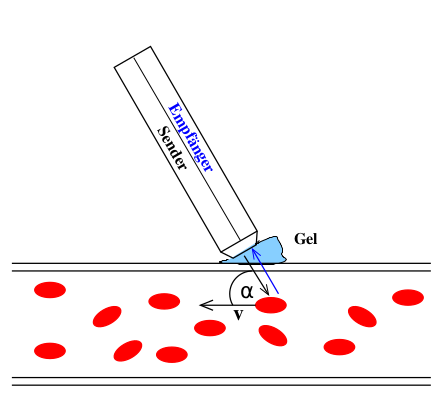
\includegraphics[scale=0.5]{content/dopplersonograph.png}
  \caption{Schematische Abbildung eines Doppler-Sonographen.}
  \label{fig:dopplersonographtheorie}
\end{figure}
\noindent
Bei dem verwendeten Versuchsaufbau mit Doppler-Prismen ergibt sich der Dopplerwinkel $\alpha$
zu
\begin{equation}
  \alpha = \SI{90}{\degree} - \arcsin( \sin{\theta} \cdot \frac{c_L}{c_P}).
  \label{eqn:gleichung5theorie}
\end{equation}
Hierbei bezeichnet $c_L$ die Schallgeschwindigkeit in der Doppler-Flüssigkeit
und $c_P$ die Schallgeschwindigkeit in dem Prismenmaterial.


\subsection{Erzeugung von Ultraschallwellen}
Die Doppler-Sonographie verwendet Ultraschallwellen. Diese haben Frequenzen
oberhalb der Schwelle des menschlichen Gehörs (zwischen $\SI{16}{\hertz}$ und
$\SI{20}{\kilo\hertz}$), also oberhalb von $\SI{20}{\kilo\hertz}$ bis $\SI{1}{\giga\hertz}$.
Die Erzeugung dieser Wellen geschieht unter Verwendung des piezo-elektrischen Effektes.
Ein piezo-elektrischer Kristall wird in einem elektrischen Feld zu Schwingungen angeregt.
Hierbei muss eine der polaren Achsen des Kristalls in Feldrichtung gerichtet sein.
Der Kristall strahlt dann Ultraschallwellen ab, welche für den Doppler-Sonographen verwendet werden.
Wenn die Anregungsfrequenz der Eigenfrequenz des Kristalls gleicht, entstehen durch Resonanz
Schwingungen mit hohen Amplituden.
Für den Empfänger des Doppler-Sonographen kann ebenfalls ein piezo-elektrischer Kristall
verwendet werden. Dabei wird der Kristall durch die einfallenden Schwingungen angeregt.
Besonders gut eignen sich Quartz-Kristalle aufgrund ihrer gleichbleibenden physikalischen
Eigenschaften, ihr piezo-elektrischer Effekt ist aber relativ gering.
